\documentclass{acm_proc_article-sp}
\bibliographystyle{unsrt}

\begin{document}

\title{Cellular Automata for Artificial Life Games}
\numberofauthors{1}
\author{
% 1st. author
%\alignauthor
%Alan S. Wang\\
%       \affaddr{Department of Bioengineering}\\
%       \affaddr{University of California}\\
%       \affaddr{California, Berkeley}\\
% 2nd. author
\alignauthor
Ian Holmes\\
       \affaddr{Department of Bioengineering}\\
       \affaddr{University of California}\\
       \affaddr{California, Berkeley}\\
       \email{ihh@berkeley.edu}
}
\date{30 November, 2013}

\maketitle
\begin{abstract}
An experimental turn-based multiplayer game framework for mobile devices is described.
Using cellular automata, the framework implements models
of condensed-matter physics, mathematical biology,
and the computational study of artificial life.
\end{abstract}

% A category with the (minimum) three required fields
%\category{H.4}{Information Systems Applications}{Miscellaneous}
%A category including the fourth, optional field follows...
%\category{D.2.8}{Software Engineering}{Metrics}[complexity measures, performance measures]


\section{Introduction}

Goal: 
build simulation game for mobile devices,
set in a persistent, multiplayer, computationally-dense world
using cellular automata ({\em CA}),
featuring models from
stochastic physics,
mathematical biology,
 and
artificial computational life ({\em A-Life})

Progress report, describing general structure of platform,
and several models from stochastic biophysics
including simulations of polymer and RNA folding kinetics.

\subsection{Cellular Automata}

CA as a platform for stochastic condensed-matter physics and biophysics
\cite{Schiff2007}

CA as a general platform for games
\cite{SimCity,DwarfFortress,Minecraft}
and electronic toys or art \cite{RuckerCAPOW,PowderToy}

\subsection{Artificial Life Models}

Electronic
\cite{VonNeumannBook,Wireworld}

Macro-biological
\cite{ConwaysLife,Langton1986}

Kinematic
\cite{Stevens2011}

Genetic algorithms
\cite{Tierra,Avida}

Core War
\cite{CoreWarGuidelines84,CoreWarDewdney85,BarkleyWaitSchmidtCoreWar2004}

\subsection{Molecular Evolution Models}

RNA World
\cite{Woese1967}
Life within vesicles.  % define 'vesicle', 'micelle'

Synthetic RNA World
\cite{PaulJoyce2002}

RNA A-Life
\cite{journals/alife/Schuster94}

RNA Folding on Lattice
\cite{LeoniVanderzande2003,JostEveraers2010,ZaraPretti2007,GillespieMayneJiang2009}

Protein folding on the lattice. HP model \cite{Dill1985,PandeRokhsar1999}

\section{Simulation}

Architecture of Cellular Automata platform.

\subsection{Low-Level Instruction Set}

Low-level (machine code):
state machines.

Synchronized and asynchronous callback.
Asynchronous guarantees callback with an exponentially-distributed wait time, scaled by particle's update rate.
Random number generator is Mersenne twister, built into board, and is replayable.

Addressing: local neighborhood.
Memory structure: 64 bits of state per cell, plus a pointer to opaque storage (can only be accessed via the supervisor scripting language).

Main 64-bit state divided into bitfields. 16 bits given over to a type field, determining how cell will be updated.
Remaining 48 bits used as dynamic storage; division into bitfields depends on the type, with some universal restrictions (e.g. bitfields cannot straddle a 32-bit boundary).
Supplemented by larger amount of read-only global storage (including global program).

The 16-bit type field selects the global program to update the cell and its neighborhood,
and also specifies a naming and sizing scheme for bitfields associated with that type's use of the dynamic storage in that cell.

The global program for a state machine mimics an ultra-minimal subset of a typical CISC architecture, generalizing the concept of the state lookup table to facilitate partial matching and rewriting of local bitfields.
The instruction set for the global program is a recognizable subset of (or easily implemented on) well-known RISC architectures, e.g. ARM\cite{seal00} and virtual game architectures, like Core War's RedCode\cite{CoreWarGuidelines84}.
The instruction set can also be quickly interpreted or implemented in C, and optimized well by C compilers.
Such details of the implementation are left opaque by design.
Code written for the low-level state machine cannot reflect on or modify its own global program.

Instruction set.
Load and Store allow access to bitfields (i.e. masking, shifting and bit-twiddling appropriately).
\\
{\bf Load-Compare-Branch} This operation essentially encapsulates memory reads. Reads a bitfield from an address, compares it to an operand, executes different code based on the result.
\\
{\bf Load-Add-Store} This operation encapsulates writes: loads a bitfield from a source address, adds an operand to it, stores in a destination address. Can optionally move or destroy the opaque storage.
\\
{\bf Random-Branch} Branches with some random probability. Random number generator replayable.
\\
{\bf Load-Switch} Analogous to C's {\tt switch} instruction: loads a bitfield from memory, and executes code based on the result. Can be implemented using Load-Compare-Branch, or internally as a jump table.
\\
{\bf Load-Register} Places a numeric constant into a register. Used in combination with indirect addressing modes of other instructions.
\\
{\bf Goto} Forward-branch to labeled routine (no backward loops).
\\
{\bf Goto-Neighbor} Branch to labeled entry point in neighbor's program (restricted to supervisor).
\\
{\bf Execute Scheme function} (restricted to supervisor).

Control flow: goto, no stack, no gosub or return.
Branches always go one way, so loops explicitly prohibited.
Program is a Directed Acyclic Graph (DAG) of finite determinable length.
Easy for server to analyze player-designed programs and maintain strong performance guarantees.
Enough flexibility for players to implement novel material properties,
as well as more sophisticated computational behaviors in the context of the grid (e.g. Turing machines, Langton ants, Wireworld-type circuits, etc.).

\subsubsection{Addressing Modes}

Several addressing modes for memory locations and operands.

Immediate vs register addressing (operands).

Indirect addressing (memory access). Registers specify cell offset, bitfield sub-address.

In principle do not need indirect or register addressing: can explicitly enumerate all cases via immediate addressing.
In practice, useful to allow some indirect and register addressing, to reduce program sizes via re-use of subroutine code.

Indirect addressing (code execution).
Goto label in neighbor's program: effectively a primitive message delivery mechanism.
Must be restricted as it can create loops.

\subsubsection{Assembly Language}

Low-level (assembly language):
Scheme. Generates (assembles) instructions for state machine.
Large built-in library for replicating patterns over Moore or von Neumann neighborhoods,
implementing reaction-diffusion models, implementing turtle-type agents, etc.

\subsection{Higher-Level Functions}

Scheme is used at a higher (supervisory) level for path-finding, goal-satisfaction, and other agent-level scripting by designers.
S-expression dynamic storage associated with each cell.

Low-level state machine can move or destroy higher-level S-expression storage, but not copy or increase it, nor read or modify its contents.

Board:
Cubic lattice.
Square slab, $S \times S \times D$.
Assuming 64-bit architecture (128 bits/cell), requires $16S^2 D$ bytes.

\subsection{Polymer State Machines}

Polymers fundamental to modeling thermodynamically fluctuating enclosures like micelles.
Also to modeling biological polymers: RNA and proteins.

Doi-Edwards theory \cite{DoiEdwards1988}

As shown in Figure~\ref{fig:polymer}.

\begin{figure}
\fbox{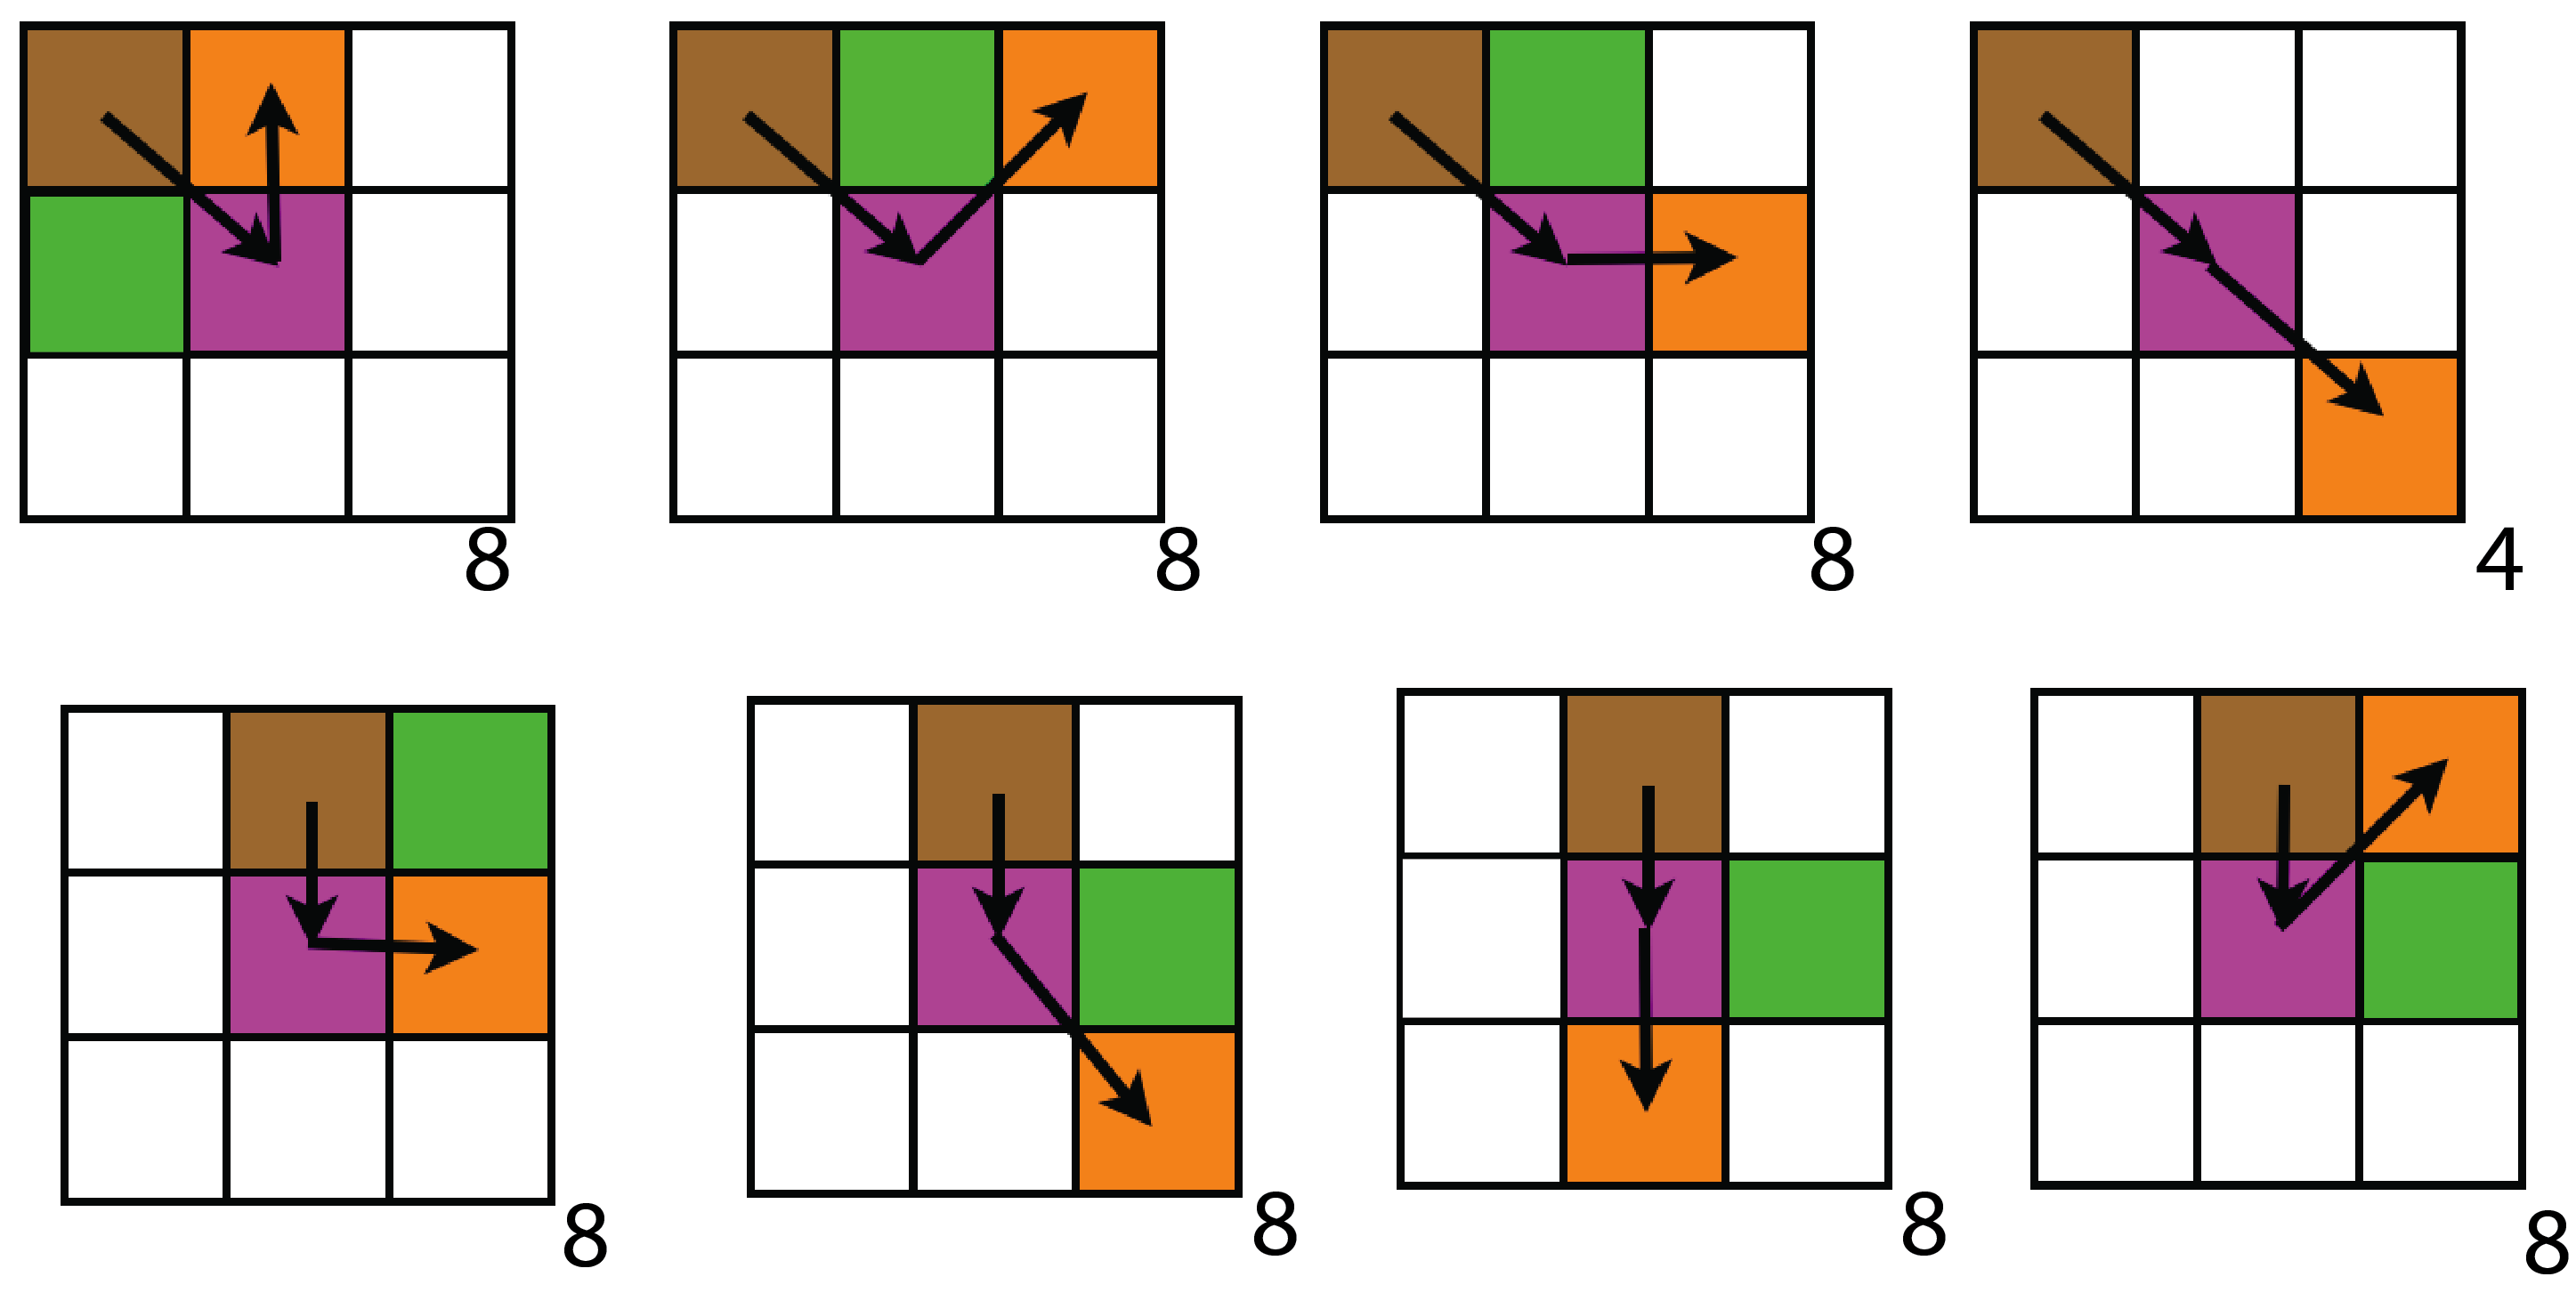
\includegraphics[width=\columnwidth]{Polymer.png}}
\caption{
\label{fig:polymer}
A few cases in the explicit automata-theoretic enumeration of polymer diffusion on the square lattice.
}
\end{figure}

Observations on model scaling:
Lookup/modify, no indirect addressing (closest thing to state tables): 2.3Mb.
Only 52k gzipped (still vicious to expand).
With indirect addressing: down to 127k (gzipped: 3k).
Scheme generator is 5k (gzipped: 1k).


\subsection{RNA State Machines}

RNA on a lattice \cite{LeoniVanderzande2003,JostEveraers2010,ZaraPretti2007,GillespieMayneJiang2009}


As shown in Figure~\ref{fig:rna}.

\begin{figure}
\fbox{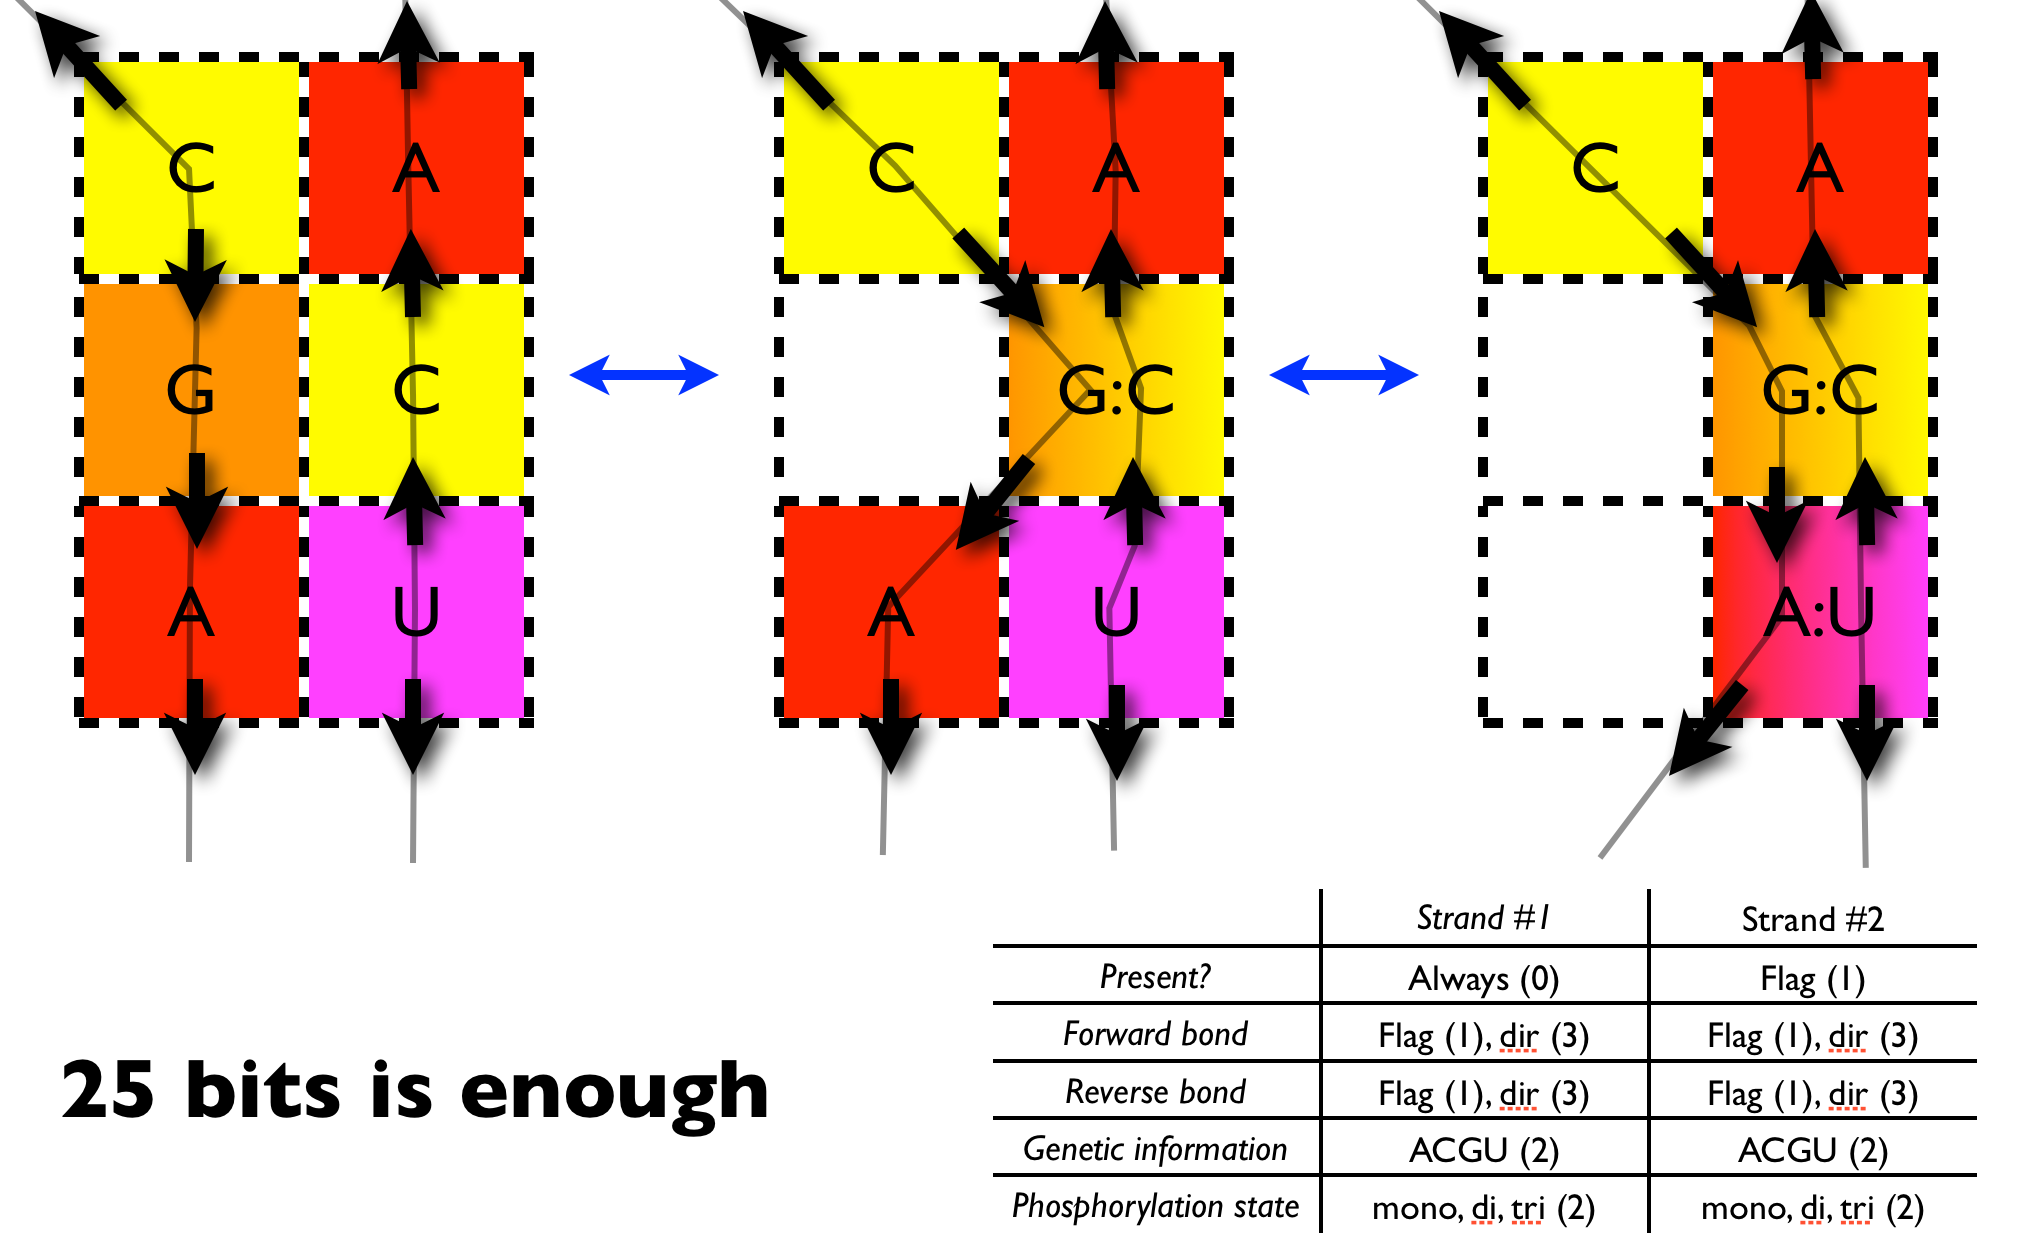
\includegraphics[width=\columnwidth]{RNA.png}}
\caption{
\label{fig:rna}
A sample case in the explicit automata-theoretic enumeration of RNA folding on the square lattice.
}
\end{figure}

\subsection{Agent State Machines}

Various agent models from above molecular length scale, used in game design.

Tumble-run: {\em E.coli}.
\cite{RosserEtAl2013}

%Sudoku ant: push obstacle a random number of blocks before changing direction.
%\cite{AntBehaviorNature}

Reaction-diffusion.
Directed diffusion.
Diffusion-limited aggregation.
\cite{DLA}

Two-dimensional square-lattice Ising model \cite{Onsager1944}.

Lotka-Volterra (predator-prey) \cite{Lotka1910,Hirota199739}.
Rock-paper-scissors games in ecology \cite{Tainaka2000}.

Ecosystem balancing and stability of food webs \cite{quince2005topological}.

Forest fires \cite{Karafyllidis1997}.

Population dynamics and spatial versions of the Wright-Fisher model \cite{MathiesonMcVean2013}.

\section{Game Design}

\subsection{Basic Play}

Terraforming simulation.
Isometric PAINT with live pixels.

Game goal: maintain dynamic equilibrium between three RPS species within a vesicle.

\subsection{Network Play}

Multiplayer implementation: RESTful server \cite{rest}.
Post lock, check board out/in.

Time-limited turns, minimum time between turns, max tool recharge per day.

Multiplayer goal: keep your population alive under attack.

Earn game-money from your population.

Client: log in/out, browse worlds, pick a world, select terraforming tools...

\subsection{Creating New Tools}

Player can POST XML to server describing new particles and tools
(with restrictions, e.g. no Scheme code at present, due partly to prohibitions on Turing-complete code transfer by App Store owners).

Spend game-money creating and using new reaction-diffusion particles and spray-tools.

Earn game-money when others buy your tools.

\subsection{Implementation}

Gnu C, libXML, GDataXML, ChibiScheme, XCode, Catalyst (Perl).

RNA state machines implemented in Java prototype.

\section{Discussion}

Work in progress.

\subsection{Acknowledgements}

Many thanks are due Alex Shinn, Richard Evans, Michael Mateas, Sean Eddy, Gerald Joyce, Chris Quince,
and Rudy Rucker for help and inspiration.


\bibliography{pzpaper}

\balancecolumns
% That's all folks!
\end{document}
